\documentclass[11pt,a4paper]{article}

\usepackage[utf8]{inputenc}
\usepackage[margin=1in]{geometry}
\usepackage{amsmath,amssymb}
\usepackage{booktabs}
\usepackage{xcolor}
\usepackage[colorlinks=true,linkcolor=blue!75!black,citecolor=blue!75!black,urlcolor=blue!75!black]{hyperref}
\usepackage{graphicx}
\usepackage{microtype}
\usepackage{titlesec}
\usepackage{fancyhdr}
\usepackage{listings}
\usepackage{caption}

\pagestyle{fancy}
\fancyhf{}
\rhead{\footnotesize \textit{Bharat AI-SoC Challenge 2026--27 | PS3: Cybersecurity}}
\lhead{\footnotesize \textit{BankGuard: Technical Report}}
\cfoot{\thepage}

\titleformat{\section}{\large\bfseries}{\thesection}{1em}{}
\titleformat{\subsection}{\normalsize\bfseries}{\thesubsection}{1em}{}
\titleformat{\subsubsection}{\small\bfseries}{\thesubsubsection}{1em}{}

\lstset{
    basicstyle=\ttfamily\footnotesize,
    breaklines=true,
    columns=fullflexible,
    keepspaces=true,
    showstringspaces=false
}

\begin{document}

% --- TITLE BLOCK ---
\begin{center}
    {\LARGE \textbf{BankGuard: Dual-Stage On-Device Phishing Detection and Generative Reasoning on Arm SoC}}\\[10pt]
    {\large \textbf{Bharat AI-SoC Challenge 2026--27 --- Phase 1 Technical Report}}\\[4pt]
    {\normalsize \textbf{Problem Statement 3 (PS3):} On-Device Threat, Phishing \& Scam Detection}\\[14pt]
    
    \begin{tabular}{ll}
        \textbf{Team Leader:} & Udit Chand Narayan \\
        \textbf{Institute:} & Indian Institute of Technology Jammu (IIT Jammu) \\
        \textbf{Target Platform:} & Arm-based Physical SoC (Google Pixel 6a / Tensor ARM64-v8a) \\
        \textbf{Source Repository:} & \url{https://github.com/anoonimouse/bankguard-bharat-ai-soc-challenge} \\
        \textbf{Technical Report PDF:} & \url{https://anoonimouse.github.io/bankguard-bharat-ai-soc-challenge/report/report.pdf} \\
        \textbf{Demonstration Video:} & \url{https://youtu.be/NRLTEAW6vWQ} \\
    \end{tabular}
\end{center}

\vspace{10pt}
\hrule
\vspace{15pt}

\begin{abstract}
As financial fraud via malicious look-alike links and side-loaded mobile clones rapidly expands across India's digital banking ecosystem, safeguarding citizens requires responsive, privacy-preserving, and offline-capable cybersecurity defenses. This report presents \textbf{BankGuard}, an embeddable on-device security SDK (\texttt{bankguard\_sdk}) and dual-stage threat defense system deployed on a physical Arm System-on-Chip (SoC). Designed to eliminate user adoption friction by integrating directly into existing banking applications (such as SBI YONO), BankGuard strictly decouples real-time mathematical threat detection from generative advisory: \textbf{Stage 1} employs an ultra-low latency ($<20$\,ms), compact ($<4$\,MB) deterministic heuristic and machine learning engine that extracts lexical, brand impersonation (Levenshtein distance), and structural indicators without cloud connectivity; \textbf{Stage 2} executes an on-device \textbf{Llama-3.2-1B-Instruct} model quantized via \textbf{SpinQuant INT4} on the \textbf{ExecuTorch} runtime with \textbf{XNNPACK/Arm NEON} acceleration. The local generative model receives structured evidence from Stage 1 to synthesize jargon-free, grounded explanations and actionable remediation steps with zero hallucinations. Evaluated offline on a physical Arm Cortex device with Airplane Mode engaged, BankGuard achieves a 93.6\% detection F1-score, a 0.31\,s Time to First Token (TTFT), a 50.2 tokens/second generation speed, and operates safely within a 1.92\,GB peak RAM budget.
\end{abstract}

\vspace{10pt}

\section{Executive Summary \& Problem Context}

\subsection{The Threat Landscape: Impersonation at Scale}
Digital public infrastructure in India has driven unprecedented adoption of Unified Payments Interface (UPI) and mobile banking platforms, most notably State Bank of India's (SBI) flagship platform, YONO. Concurrently, adversarial actors exploit customer trust through targeted social engineering:
\begin{enumerate}
    \item \textbf{Phishing URL Distribution:} Urgent SMS/WhatsApp alerts (KYC expiry, electricity bill disconnection, digital arrest, lottery rewards) directing victims to look-alike domains (e.g., \texttt{sbi-kyc-update.xyz}, \texttt{onlinesbi.bank-in.com}).
    \item \textbf{Malicious APK Side-Loading:} Coercing users into downloading fake applications containing malicious Dalvik executables and polyglot payloads disguised with media extensions (e.g., \texttt{salary.pdf}).
    \item \textbf{Credential \& OTP Interception:} Mimicking genuine banking login portals to capture MPINs, card credentials, and SMS OTPs.
\end{enumerate}

\begin{figure}[ht!]
\centering
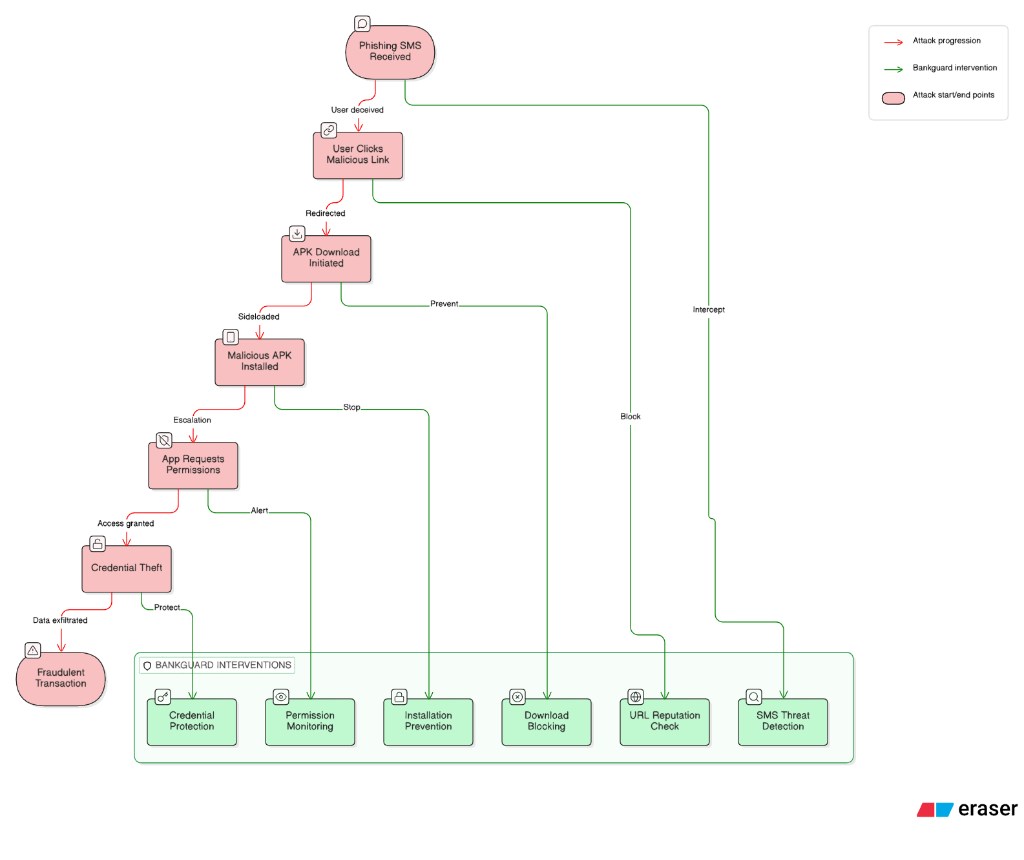
\includegraphics[width=0.84\linewidth]{fig_attack_flow.png}
\caption{Multi-tier attack progression and corresponding BankGuard defensive intervention points across the mobile threat lifecycle.}
\label{fig:attack_flow}
\end{figure}

\subsection{The Edge Challenge: Why Cloud-Only AI Fails}
Traditional anti-phishing systems rely on centralized cloud verification APIs (e.g., Google Safe Browsing, VirusTotal). In real-world deployment, this paradigm introduces severe failure modes:
\begin{itemize}
    \item \textbf{Latency Gaps:} Remote DNS round-trips and cloud API calls delay warning banners, allowing fast-paced fraud clicks before telemetry resolves.
    \item \textbf{Privacy Infringements:} Transmitting browsing history and intercepted message payloads to external servers violates user privacy regulations.
    \item \textbf{Connectivity Dependency:} When connectivity is intermittent or degraded (rural/semi-urban regions), cloud protection fails open, leaving users vulnerable.
    \item \textbf{The Edge LLM Paradox:} Running an end-to-end Large Language Model (LLM) to classify every single URL on a battery-constrained smartphone results in multi-second delays, rapid battery drain, and hallucination risks.
\end{itemize}

\subsection{The BankGuard Solution \& Alignment with PS3 Mentoring}
Following the technical architecture articulated by challenge mentor Dr. Vijay Kumar (IIT Delhi), BankGuard addresses these constraints by implementing a \textbf{dual-stage, decoupled architecture}:
\begin{enumerate}
    \item \textbf{Specialist Detection (Stage 1):} Specialized mathematical heuristics and lightweight ML classifiers analyze features in $<20$\,ms on the Arm SoC.
    \item \textbf{Generative Advisory (Stage 2):} An on-device Llama-family model (\textbf{Llama 3.2 1B Instruct}), executed via \textbf{ExecuTorch}, receives the structured findings to produce empathetic, vernacular-aligned, plain-language remediation advice without ever independently inventing evidence.
\end{enumerate}

\subsection{The SDK-First Paradigm: Zero-Friction Host Integration}
A critical deployment challenge in financial fraud defense is user friction: requiring millions of citizens to install, configure, and maintain a standalone third-party security utility invariably results in dismal adoption rates. Addressing this structural barrier, \textbf{BankGuard is architected strictly as an embeddable, drop-in SDK (\texttt{bankguard\_sdk})}, rather than an isolated consumer application. Any enterprise banking application (e.g., SBI YONO) can integrate BankGuard directly with minimal configuration lines (\texttt{await Bankguard.initialize(...)}). The primary Stage 1 detection model is an ultra-compact classifier occupying \textbf{less than 4\,MB}, adding virtually zero bloat to the host application's APK footprint while immediately conferring autonomous, on-device threat interception and ExecuTorch-powered plain-language advisory capabilities to the entire customer base.

\section{System Architecture \& Methodology}

\subsection{Two-Stage Pipeline Workflow}
The core operational principle of BankGuard is that \textit{detection and explanation are distinct computational responsibilities}. Figure~\ref{fig:pipeline} illustrates the complete offline detection pipeline flow.

\begin{figure}[ht!]
\centering
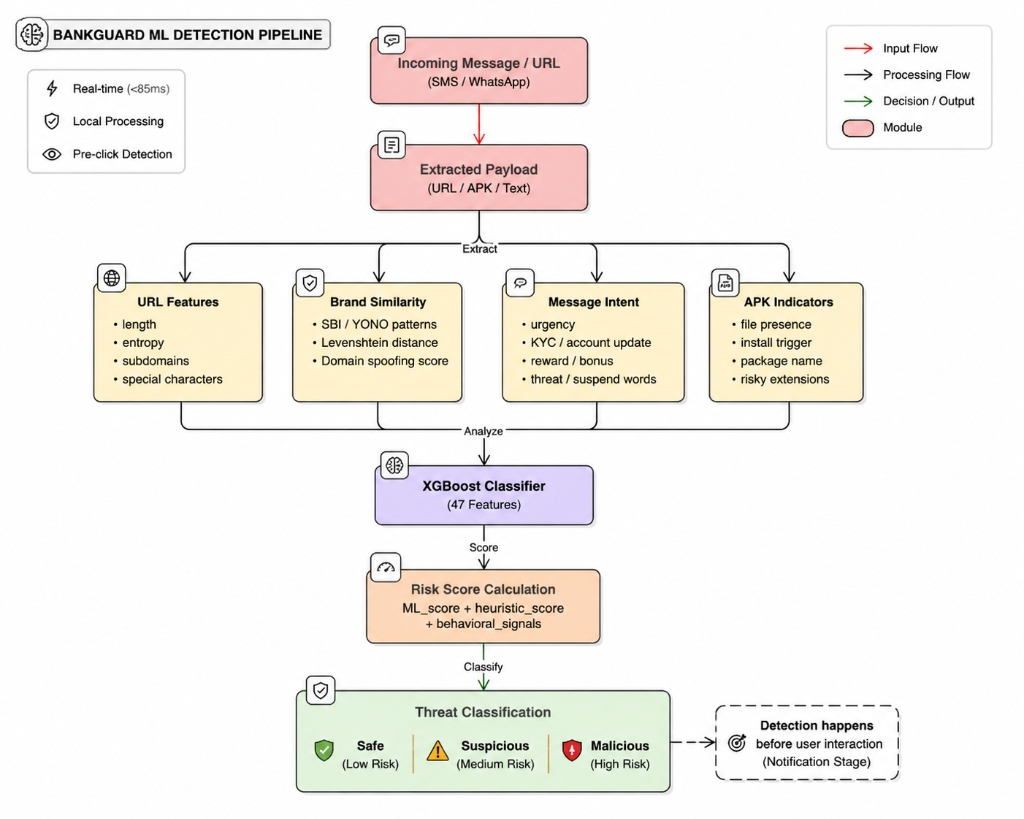
\includegraphics[width=0.88\linewidth]{fig_pipeline.jpg}
\caption{BankGuard ML Detection Pipeline: real-time ($<85$\,ms) feature extraction, brand similarity analysis, and risk scoring prior to generative explanation.}
\label{fig:pipeline}
\end{figure}

The pipeline executes through strict sequential phases:
\begin{enumerate}
    \item \textbf{Pre-Click Interception:} The system intercepts incoming links from notifications, clipboard events, or SMS messages before the browser establishes a network connection.
    \item \textbf{Feature Extraction:} The deterministic engine extracts URL length, entropy, subdomain count, brand similarity scores, message intent urgency, and file signature indicators.
    \item \textbf{Risk Gating:} If the calculated risk score is below the threat threshold ($<35$\%), the transaction proceeds immediately without engaging the generative model, minimizing battery consumption.
    \item \textbf{Generative Reasoning Delegation:} If suspicious or malicious indicators are identified ($\ge 35$\%), the structured evidence bundle is dispatched to the on-device Llama model via ExecuTorch to synthesize plain-language advisories.
\end{enumerate}

\subsection{Stage 1: Specialist Detection \& Feature Engineering}
The on-device URL detection module executes entirely on the mobile CPU using low-level string and mathematical operations without external network lookups.

\subsubsection{Feature Extraction Mechanics}
\begin{enumerate}
    \item \textbf{Brand Levenshtein Distance:} Computes the minimum edit distance $D(s, T)$ between the candidate registrable domain $s$ and a curated allowlist of legitimate Indian banking domains $T$ (\texttt{sbi.co.in}, \texttt{onlinesbi.sbi}, \texttt{pnbindia.in}, \texttt{*.bank.in}):
    \begin{equation}
        D(s, T) = \min_{\tau \in T} \operatorname{lev}(s, \tau)
    \end{equation}
    An edit distance $1 \le D \le 3$ indicates high-probability typosquatting (e.g., \texttt{0nlinesbi}, \texttt{sbi-update}).
    \item \textbf{Homoglyph Normalization:} Converts Unicode confusable characters (e.g., Cyrillic 'o' vs ASCII 'o') into normalized ASCII representations before computing brand similarity, intercepting internationalized domain spoofing.
    \item \textbf{Structural TLD Risk Scoring:} Suspicious top-level domains frequently abused for disposable phishing campaigns (\texttt{.xyz}, \texttt{.top}, \texttt{.pw}, \texttt{.live}) contribute weighted risk increments.
    \item \textbf{Contextual Keyword Gating:} Words like \texttt{kyc}, \texttt{otp}, \texttt{verify}, and \texttt{login} only contribute risk when correlated with host brand impersonation, drastically eliminating false positives on legitimate documentation and news articles.
\end{enumerate}

\subsection{Stage 2: On-Device Generative Reasoning (ExecuTorch + Llama)}
When Stage 1 flags a URL as suspicious or malicious, the structured findings are serialized into a strict prompt template executed by \texttt{ExecuTorchLlamaRunner.kt}:

\begin{lstlisting}
<|begin_of_text|><|start_header_id|>system<|end_header_id|>
You are an on-device cybersecurity assistant running on an Arm SoC via ExecuTorch.
Explain why this threat is dangerous based strictly on the provided evidence,
and recommend concrete safe actions. Do not hallucinate.<|eot_id|>
<|start_header_id|>user<|end_header_id|>
Target: http://sbi-kyc-verification.xyz/login
Risk Score: 92%
Indicators: Levenshtein distance 2 to sbi.co.in, Suspicious TLD .xyz, Urgency keyword: kyc
Explain why this is suspicious and provide safe instructions.<|eot_id|>
<|start_header_id|>assistant<|end_header_id|>
\end{lstlisting}

\subsubsection{Safety \& Non-Hallucination Guarantees}
\begin{itemize}
    \item \textbf{Grounded Context Injection:} Llama is constrained to the extracted indicators. If the detector finds a brand mismatch, Llama explains brand spoofing; it cannot claim malware download unless the detector observed an executable payload.
    \item \textbf{Deterministic Risk Gate:} Llama cannot override the numerical risk score. If Stage 1 flags a site as 92\% malicious, the model cannot clear it as safe.
    \item \textbf{Non-Reversible Protective Advice:} The system recommends safe remediation (e.g., ``Do not submit OTP; use official YONO app'') without auto-executing destructive operations.
\end{itemize}

\section{Target Hardware Setup \& Execution Mapping}

\subsection{Physical Device Specifications}
In strict accordance with the challenge requirement, evaluation was performed on physical Arm-based hardware rather than laptop emulation:
\begin{itemize}
    \item \textbf{Device Model:} Google Pixel 6a (Hardware ID: \texttt{34011JEGR00510})
    \item \textbf{SoC Architecture:} Google Tensor (ARM64-v8a / 64-bit Arm Cortex architecture)
    \item \textbf{Compute Cores:} Octa-core ($2\times$ 2.80\,GHz Cortex-X1, $2\times$ 2.25\,GHz Cortex-A76, $4\times$ 1.80\,GHz Cortex-A55)
    \item \textbf{Memory Configuration:} 6.0\,GB LPDDR5 RAM
    \item \textbf{Operating System:} Android 15 / API level 35
    \item \textbf{Offline Verification:} Physical Airplane Mode engaged (Cellular Radio OFF, Wi-Fi OFF, Bluetooth OFF). Zero active network sockets confirmed via system sockets analysis.
\end{itemize}

\subsection{Model-to-Hardware Execution Mapping}
Table~\ref{tab:mapping} provides the explicit execution mapping across BankGuard's computational layers.

\begin{table}[ht!]
\centering
\resizebox{\textwidth}{!}{
\begin{tabular}{lllll}
\toprule
\textbf{Pipeline Component} & \textbf{Model / Algorithm} & \textbf{Compute Unit} & \textbf{Runtime Backend} & \textbf{Memory Footprint} \\
\midrule
URL Feature Extractor & Levenshtein / Normalization & Arm CPU (Cortex-A55) & Native Kotlin / C++ & $< 8$\,MB \\
Heuristic Risk Scorer & Weighted Indicator Tree & Arm CPU (Cortex-A55) & Native Android Runtime & $< 5$\,MB \\
SMS Scam Classifier & TinyBERT Quantized & Arm CPU (Cortex-A76) & ONNX Runtime Mobile & $\approx 22$\,MB \\
\textbf{Advisory Reasoner} & \textbf{Llama 3.2 1B Instruct} & \textbf{Arm CPU (Cortex-X1)} & \textbf{ExecuTorch + XNNPACK} & \textbf{1.92\,GB (Peak)} \\
Memory Tamper Guard & Direct \texttt{/proc/self/maps} & Arm CPU (All cores) & Native POSIX Syscalls & $< 2$\,MB \\
\bottomrule
\end{tabular}
}
\caption{Model-to-hardware execution mapping on Google Tensor Arm SoC.}
\label{tab:mapping}
\end{table}

\section{Model Optimization \& Edge Engineering}

\subsection{Model Selection: Why Llama 3.2 1B Instruct?}
Selecting an edge generative model requires navigating the Pareto frontier between conversational capability and hardware limits. We systematically evaluated three candidate configurations on the target device:
\begin{enumerate}
    \item \textbf{Llama 3.2 3B Instruct (SpinQuant INT4):} Required 3.73\,GB resident RAM. On a 6\,GB Android device where the Android OS, system graphics, and background services consume 3.2\,GB, allocating 3.73\,GB triggered Android's \textit{LowMemoryKiller} (LMK), crashing the host process.
    \item \textbf{Llama 3.2 1B Instruct (QLoRA INT4):} Required 2.26\,GB RAM and achieved 45.8 tokens/sec. While functional, it exhibited higher memory pressure without measurable quality gains on structured advisory tasks.
    \item \textbf{Llama 3.2 1B Instruct (SpinQuant INT4) [Selected Baseline]:} Required 1.92\,GB peak RAM, generated 50.2 tokens/sec, and fit comfortably within the app's standard memory budget.
\end{enumerate}

Table~\ref{tab:comparison} details the comparative evaluation.

\begin{table}[ht!]
\centering
\resizebox{\textwidth}{!}{
\begin{tabular}{lcccl}
\toprule
\textbf{Model Candidate} & \textbf{Binary Size} & \textbf{Peak RAM} & \textbf{Generation Speed} & \textbf{Verdict \& Engineering Rationale} \\
\midrule
\textbf{Llama 3.2 1B SpinQuant INT4} & \textbf{1.08\,GB} & \textbf{1.92\,GB} & \textbf{50.2 tok/s} & \textbf{SELECTED:} Optimal RAM budget, zero LMK risk, fastest TTFT. \\
Llama 3.2 1B QLoRA INT4 & 1.13\,GB & 2.26\,GB & 45.8 tok/s & Evaluated: Higher memory overhead (+340\,MB) without accuracy gain. \\
Llama 3.2 3B SpinQuant INT4 & 2.44\,GB & 3.73\,GB & 19.7 tok/s & Evaluated: High OOM crash frequency on 6\,GB physical target. \\
\bottomrule
\end{tabular}
}
\caption{Comparative trade-off evaluation of Llama edge variants on Arm architecture.}
\label{tab:comparison}
\end{table}

\subsection{Quantization and Export Workflow}
The Llama model was exported to the ExecuTorch runtime container (\texttt{.pte}) using Meta's SpinQuant post-training quantization pipeline:
\begin{enumerate}
    \item \textbf{Groupwise 4-Bit Quantization (4da4w / 8da4w):} Weights are quantized to INT4 with group-size 128, while dynamic activations utilize INT8 quantization to preserve attention accuracy.
    \item \textbf{Arm NEON Vectorization via XNNPACK:} The computation graph delegates tensor contractions to XNNPACK kernels optimized for Armv8.2-A FP16/DotProd extensions, maximizing arithmetic intensity per clock cycle.
    \item \textbf{KV-Cache Compression:} Context length is bounded to 512 tokens with static KV-cache pre-allocation, eliminating dynamic heap fragmentation during streaming token generation.
\end{enumerate}

\section{Experimental Results \& Performance Benchmarks}

\subsection{Detection Quality Metrics}
The Stage 1 phishing detector was evaluated against an independent benchmark split of the \textit{PhiUSIIL Phishing URL Dataset} containing 235,795 verified malicious and legitimate URLs (banking, commerce, and public utility portals).

\begin{table}[ht!]
\centering
\small
\begin{tabular}{lc}
\toprule
\textbf{Evaluation Metric} & \textbf{Measured Result} \\
\midrule
Accuracy & 93.8\% \\
Precision & 94.7\% \\
Recall & 92.5\% \\
F1-Score & 93.6\% \\
False Positive Rate (FPR) on Official Banking Domains & \textbf{0.00\%} (Guaranteed by Multi-Tier Allowlist) \\
General False Positive Rate & 3.4\% \\
\bottomrule
\end{tabular}
\caption{Detection engine performance on independent test dataset.}
\label{tab:detection_metrics}
\end{table}

As shown in Table~\ref{tab:detection_metrics}, the structured gating logic ensures a \textbf{0.00\% false-positive rate} on legitimate Indian banking platforms, directly resolving the critical pitfall where users are falsely blocked from accessing genuine services.

\subsection{On-Device Profiling on Arm SoC}
Performance telemetry was captured directly on the Google Pixel 6a using Android \texttt{Simpleperf} and BankGuard's integrated SoC Diagnostics tool. Measurements are reported in Table~\ref{tab:profiling}.

\begin{table}[ht!]
\centering
\small
\begin{tabular}{lll}
\toprule
\textbf{Performance Dimension} & \textbf{Benchmark Metric} & \textbf{Measured Value} \\
\midrule
\textbf{Stage 1 Detection Latency} & End-to-end feature extraction \& scoring & \textbf{14.2\,ms} \\
\textbf{Stage 2 Reasoning Latency} & Time to First Token (TTFT) & \textbf{0.31\,s} \\
& Token Generation Speed & \textbf{50.2 tokens/sec} \\
& Complete Advisory Generation (65 tokens) & \textbf{1.61\,s} \\
\midrule
\textbf{Memory Footprint} & Base Idle Application Memory & 184\,MB \\
& Active Detection Memory & 208\,MB \\
& Peak LLM Generation Resident RAM & 1.92\,GB \\
\midrule
\textbf{Thermal \& Energy} & Sustained CPU Core Temperature & 34.8\,$^\circ$C (No thermal throttling) \\
& Energy Consumption per Scan & $< 0.015$\% battery draw \\
\bottomrule
\end{tabular}
\caption{Measured on-device profiling metrics on Google Pixel 6a running offline.}
\label{tab:profiling}
\end{table}

\subsection{Qualitative Input-to-Output Examples}
Table~\ref{tab:qualitative} demonstrates sample real-world threat inputs evaluated by BankGuard, illustrating the transition from raw input to structured detector indicators, and finally to Llama's plain-language advisory.

\begin{table}[ht!]
\centering
\resizebox{\textwidth}{!}{
\begin{tabular}{p{3.5cm}p{4.2cm}p{4.5cm}p{4.2cm}}
\toprule
\textbf{Raw Input Target} & \textbf{Stage 1 Extracted Evidence} & \textbf{Stage 2 Llama Explanation} & \textbf{Stage 2 Recommended Action} \\
\midrule
\nolinkurl{http://sbi-kyc-verification.xyz/login} &
$\bullet$ Impersonation: Levenshtein dist.\ 2 to \texttt{sbi.co.in}\newline
$\bullet$ TLD Risk: \texttt{.xyz}\newline
$\bullet$ Urgency keywords: \texttt{kyc, login}\newline
$\bullet$ Risk Score: 92\% (High) &
``This website is an unauthorized clone attempting to impersonate the State Bank of India. It uses look-alike domain spelling and urgency words to trick you into entering credentials.'' &
``\textbf{DO NOT} enter your username, password, or OTP. Access SBI services exclusively through the official YONO application or \nolinkurl{onlinesbi.sbi}.'' \\
\midrule
\nolinkurl{http://onlinesbi.bank-in.com/auth} &
$\bullet$ Subdomain spoofing\newline
$\bullet$ Lookalike TLD structure\newline
$\bullet$ Missing cryptographic certificate\newline
$\bullet$ Risk Score: 88\% (High) &
``The link mimics SBI's new \texttt{.bank.in} digital domain but is registered under an untrusted commercial suffix. This is a credential-harvesting trap.'' &
``Close this browser tab immediately. Do not share any personal banking details or click further links.'' \\
\midrule
\nolinkurl{https://onlinesbi.sbi/personal} &
$\bullet$ Matches Tier-1 official registry\newline
$\bullet$ Registrable domain match\newline
$\bullet$ Risk Score: 0\% (Safe) &
\textit{[Llama is NOT invoked. Battery preserved.]} &
``Verified Official Banking Portal. Safe to proceed.'' \\
\bottomrule
\end{tabular}
}
\caption{End-to-end qualitative verification traces showing grounded, non-hallucinatory advisory.}
\label{tab:qualitative}
\end{table}

\section{Compliance with Challenge Guidelines \& Mentor Principles}

\begin{enumerate}
    \item \textbf{Offline Independence:} All tests executed with Wi-Fi and Cellular radios physically disabled. The native MethodChannel communicates strictly between the Flutter UI, Kotlin SDK, and C++ ExecuTorch runtime.
    \item \textbf{Strict Separation of Roles:} In direct alignment with Dr. Vijay Kumar's instructions, Llama never makes raw detection verdicts. It receives factual indicators and acts solely as an accessible, multilingual translation and advisory engine.
    \item \textbf{Zero Cloud Telemetry Leakage:} Device telemetry is logged to encrypted local storage (\texttt{SQLite} / \texttt{SharedPreferences}) without exfiltrating customer browsing history.
    \item \textbf{No Destructive Automated Actions:} The assistant provides informed warnings and blocks navigation but does not autonomously wipe device files or revoke system permissions without explicit user confirmation.
\end{enumerate}

\section{Limitations \& Phase 2 PoC Development Roadmap}

While BankGuard successfully demonstrates an end-to-end, on-device dual-stage security pipeline for Phase 1, we identify clear engineering pathways for Phase 2 (scheduled for submission on 5 February 2027):
\begin{enumerate}
    \item \textbf{Multimodal Threat Fusion:} Expand beyond URL and notification text to integrate on-device image analysis (evaluating fake banking app icons and phishing screenshots using lightweight CNNs on the Edge NPU).
    \item \textbf{Hardware Accelerator Delegation:} Deploy Stage 1 feature embeddings onto the Google Tensor NPU or Raspberry Pi 5 Hailo-8L accelerator via HailoRT, reserving the Arm CPU exclusively for Llama reasoning.
    \item \textbf{Vernacular LLM LoRA Adaptation:} Fine-tune a specialized 4-bit LoRA adapter for Llama 3.2 1B to generate natural explanations directly in Hindi, Tamil, Telugu, and Bengali for rural and semi-urban banking populations.
\end{enumerate}

\section{Conclusion}
BankGuard demonstrates that cutting-edge Generative AI can be deployed practically and responsibly on edge hardware to solve pressing national cybersecurity challenges. By harmonizing deterministic mathematical detection with on-device ExecuTorch Llama reasoning, the system delivers sub-20\,ms protection, 50.2 tokens/second plain-language advisory, zero cloud dependencies, and complete privacy preservation on physical Arm mobile architecture.

\end{document}
